\newpage
\section{Methodology} \label{Section:Methodology}

%In this part, we will describe everything needed to realise the survey and reproduce the same data. Let's start with the GPR setup we use.

\subsection{GPR Setup}

\begin{wrapfigure}[27]{l}{0.5\linewidth}
    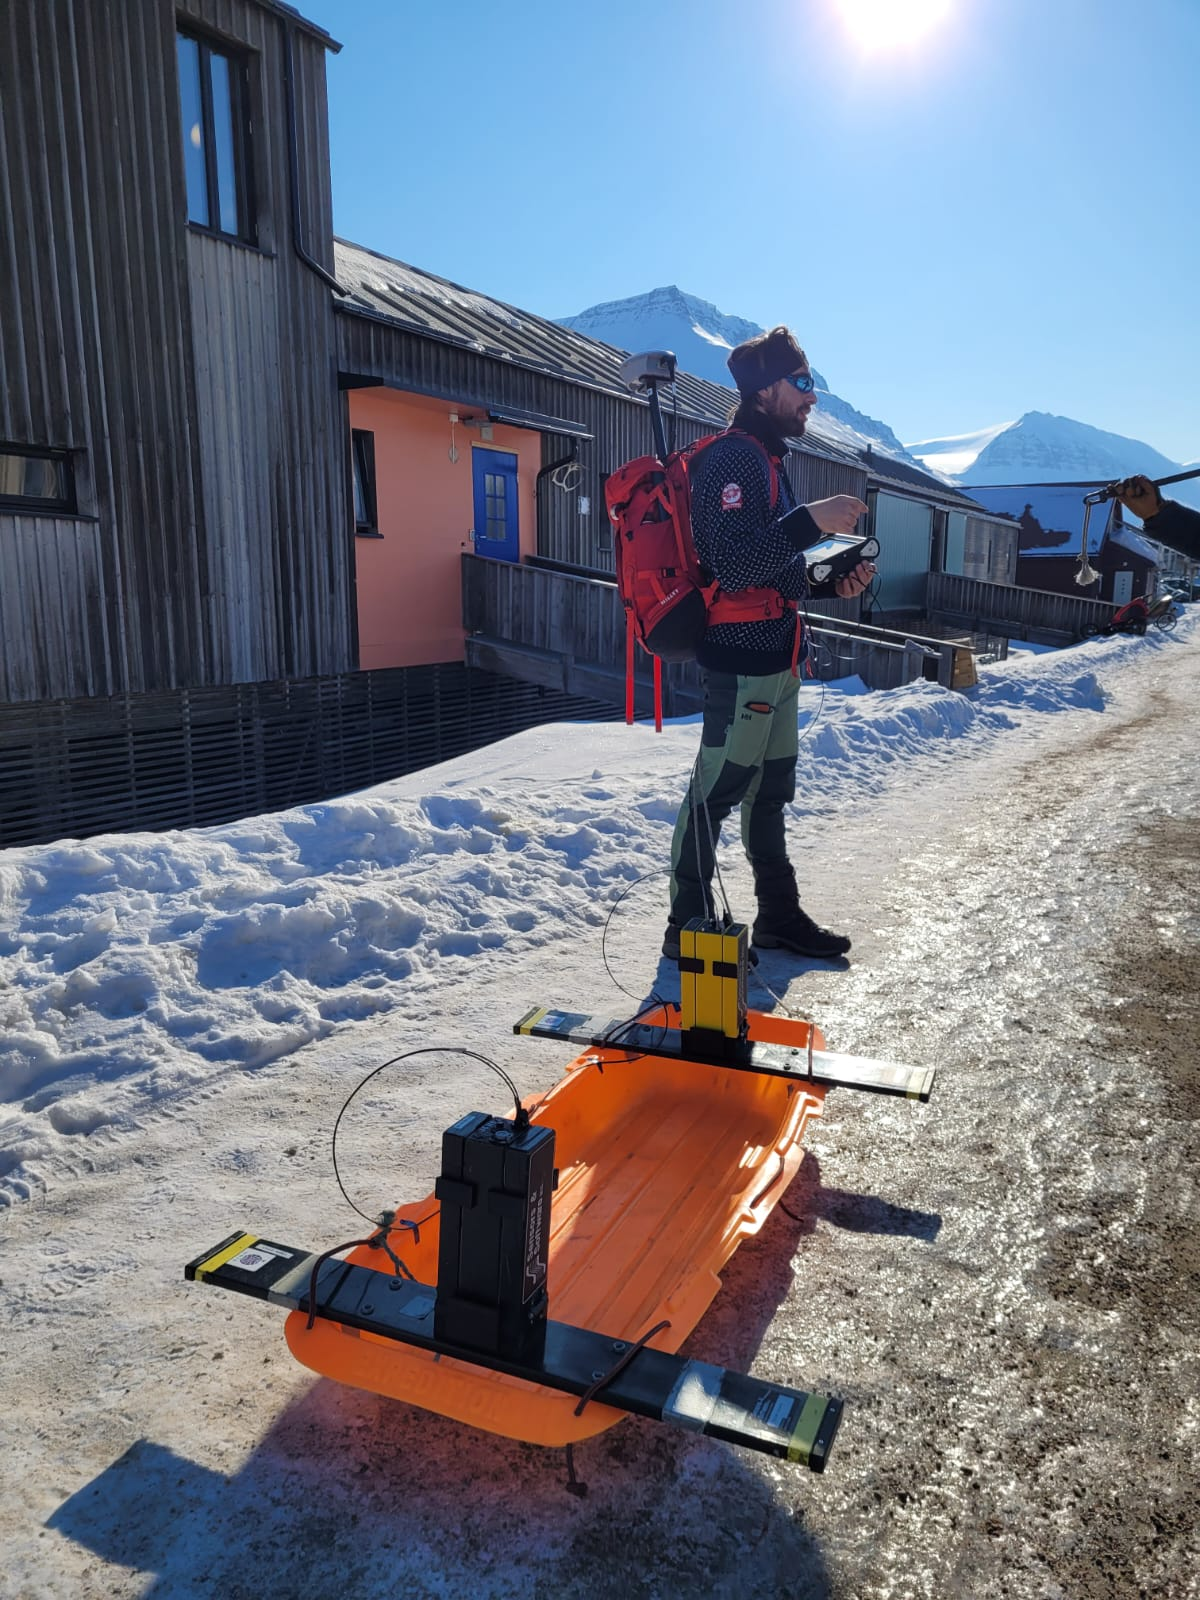
\includegraphics[width=\linewidth]{Images/00_Methodology/PictureGunnhild.jpg}
    \caption{GRP setup used for the survey during the tests (see \ref{Subsection:TestSurvey}) realised in the main street of Longyearbyen. \emph{Photo : Gunnhild Næss - UNIS}}
    \label{fig:PictureGunnhild}
\end{wrapfigure}

The setup to run a GPR in a steep slope as described in \ref{Paragraph:SiteDescription} should be easy to carry and quite compact but compelling with all the requirements of the GPR. The picture on figure \ref{fig:PictureGunnhild} shows all the elements as listed bellow.



\begin{itemize}
    \item \emph{The pulk} will be the support for the GPR receiver and transmitter. The challenge is to fix both antennae on it and the simpler solution was to tape the antenna on the pulk.
    \item \emph{The antennas} placed directly above the pulk (rectangular black plate)
    \item \emph{The transmitter}, black box above the back antenna on the figure, \ref{fig:PictureGunnhild} will generate the signal send by a fiber optic from the DVL\footnote{Data logger}. The transmitter we used requires to disconnect the output wire.
    \item \emph{The receiver}, yellow box above the front antenna, will be the most critical part of the set up. The receiver which receives reflection signal from the ground is also the most sensitive to all external perturbations. That is why for the 'real' survey, we chose to invert the receiver and the transmitter to keep the receiver the furthest away from all other electronics devices.
\end{itemize}

\begin{itemize}
    \item \emph{The GPS receiver} located on the top of the backpack will allow to have the position of each measurements and to correct the position of the lines during the processing. It will also give the indication about the elevation which is very important during a slope survey.
    \item \emph{The DVL} will receive and send all the data and save it. It also allows to set up the whole GPR (Frequency, Antenna separation... as presented in \ref{SubSection:settings})
\end{itemize}



\subsection{Test survey} \label{Subsection:TestSurvey}


In order to try the whole setup which was new (especially the data logger), we went in the streets of Longyearbyen to draw few lines for tests. This survey allows to fix few issues with the GPS and to improve the organisation of the receiver and the transmitter for the "real survey". During these preliminary tests, Gunnhild Næss took a picture presented on figure \ref{fig:PictureGunnhild}. We only present one of the lines performed during this survey because it is very characteristics of a buried pipe (see figure \ref{fig:testLine} in the \ref{section:result}).

\newpage
\subsection{Field work organisation}

\begin{wrapfigure}[17]{r}{0.4\textwidth}
    \centering
    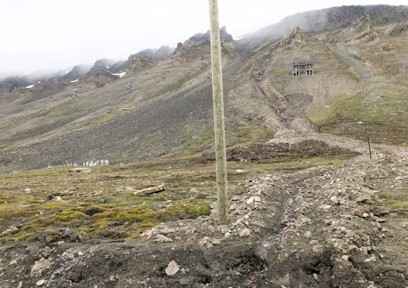
\includegraphics[width=0.38\textwidth]{Images/00_Methodology/LandSlide2018.jpg}
    \caption{Landslide in Longyearbyen in 2018 \emph{Photo: Alexander Lembke} \cite{Landslide2018Longyeabyen}}
    \label{fig:Landslide2018}
\end{wrapfigure}

\paragraph{Site description} \label{Paragraph:SiteDescription}

One of the key concern in Longyearbyen is the safety of people and in the recent years few major events happened. One of the most important was the avalanche in 2015 which killed 2 people and destroyed many houses. In 2018, a landslide went down on the side of Platåberget and crossed the road close to the cemetery. Even if no one was injured, it was obvious that a system to monitore the permafrost and the conditions around the town was required in order to prevent any serious event. This project is the PermaMeteoCommunity \cite{PermaMeteoCommunity} which creates a model to predict event such as landslides. That is why we chose to do a survey close to the borehole which are used to monitor the temperature of the permafrost where the landslide happened in 2018. The localisation of the area is shown on figure \ref{fig:Location}.




\begin{figure}
    \centering
    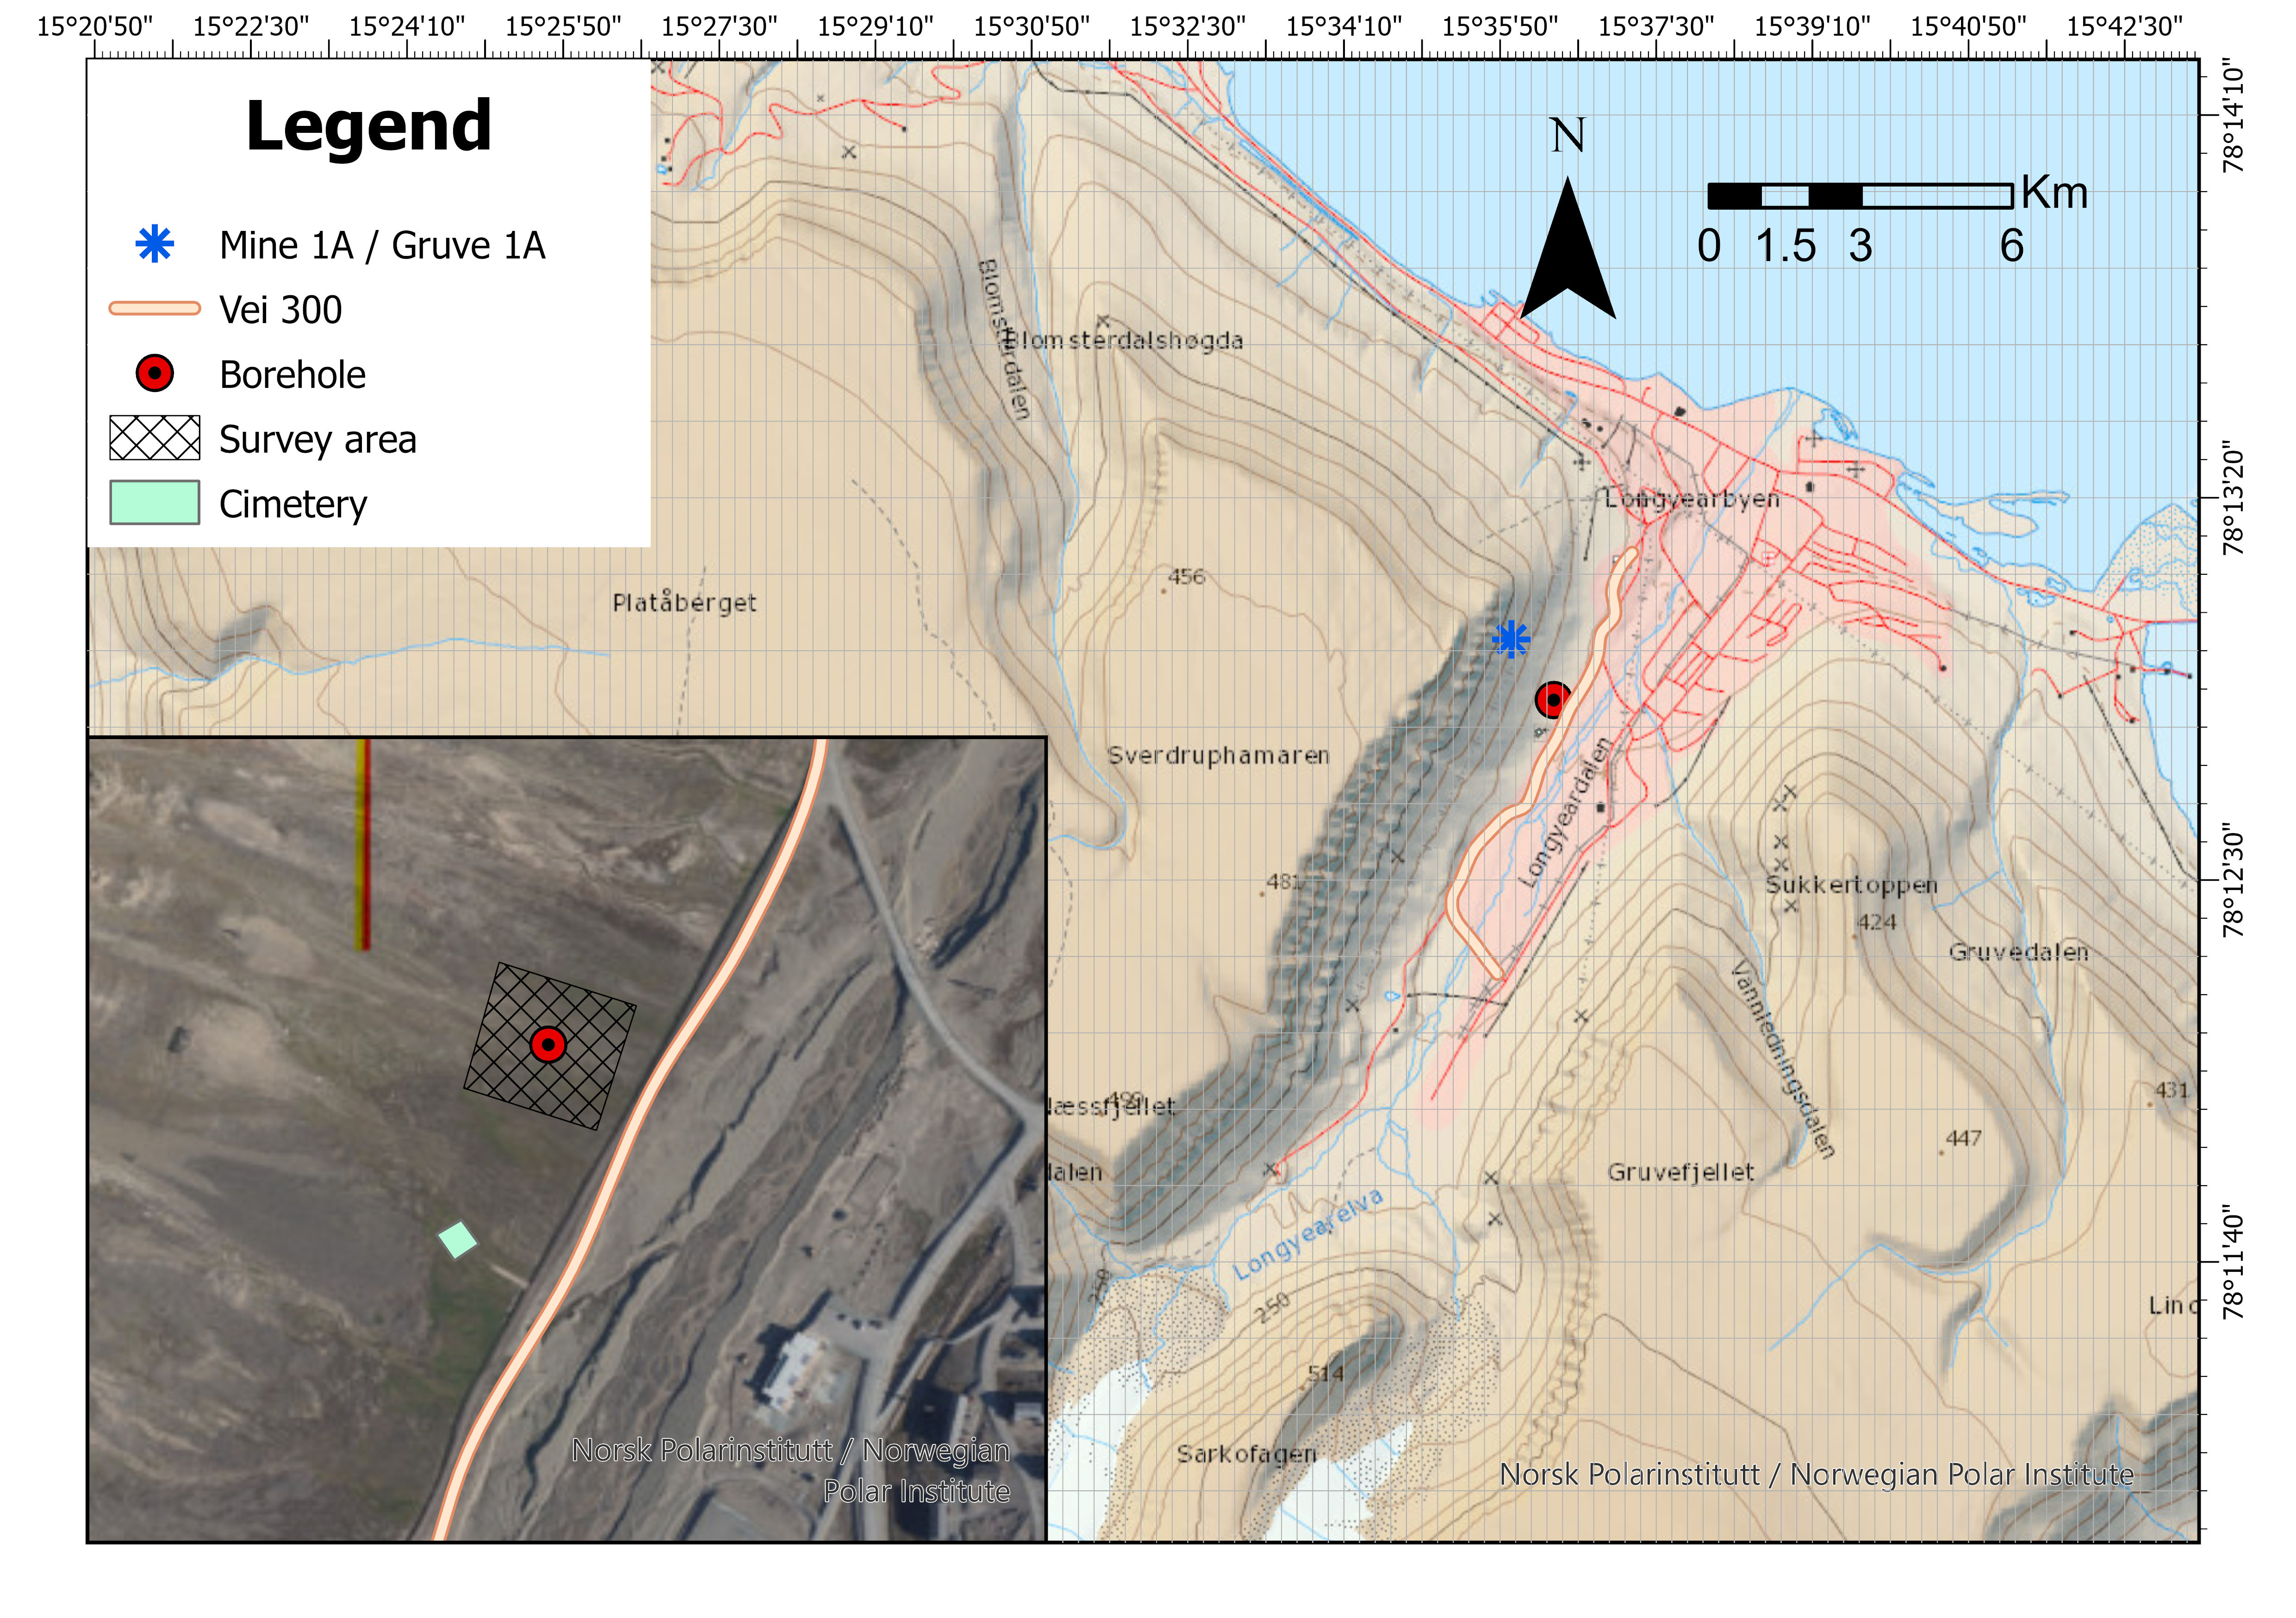
\includegraphics[width=\linewidth]{Images/00_Methodology/GeographicSituation.jpg}
    \caption{Location of the survey area in Longyearbyen}
    \label{fig:Location}
\end{figure}


\paragraph{Geology} Using a GPR as for goal to "see" the subsurface and also some geological consideration are required. We had the information from the survey on the Geological map of Svalbard \cite{Atakan2015GeoscienceSvalbard} and the result is presented on figure \ref{fig:GeologicalBackground}. This map gives us the information that the bedrock will be most likely sandstone and shale which give us an information about the expected velocity around 0.130 m/ns \cite{GPRAnalysis}.

\begin{figure}
    \centering
    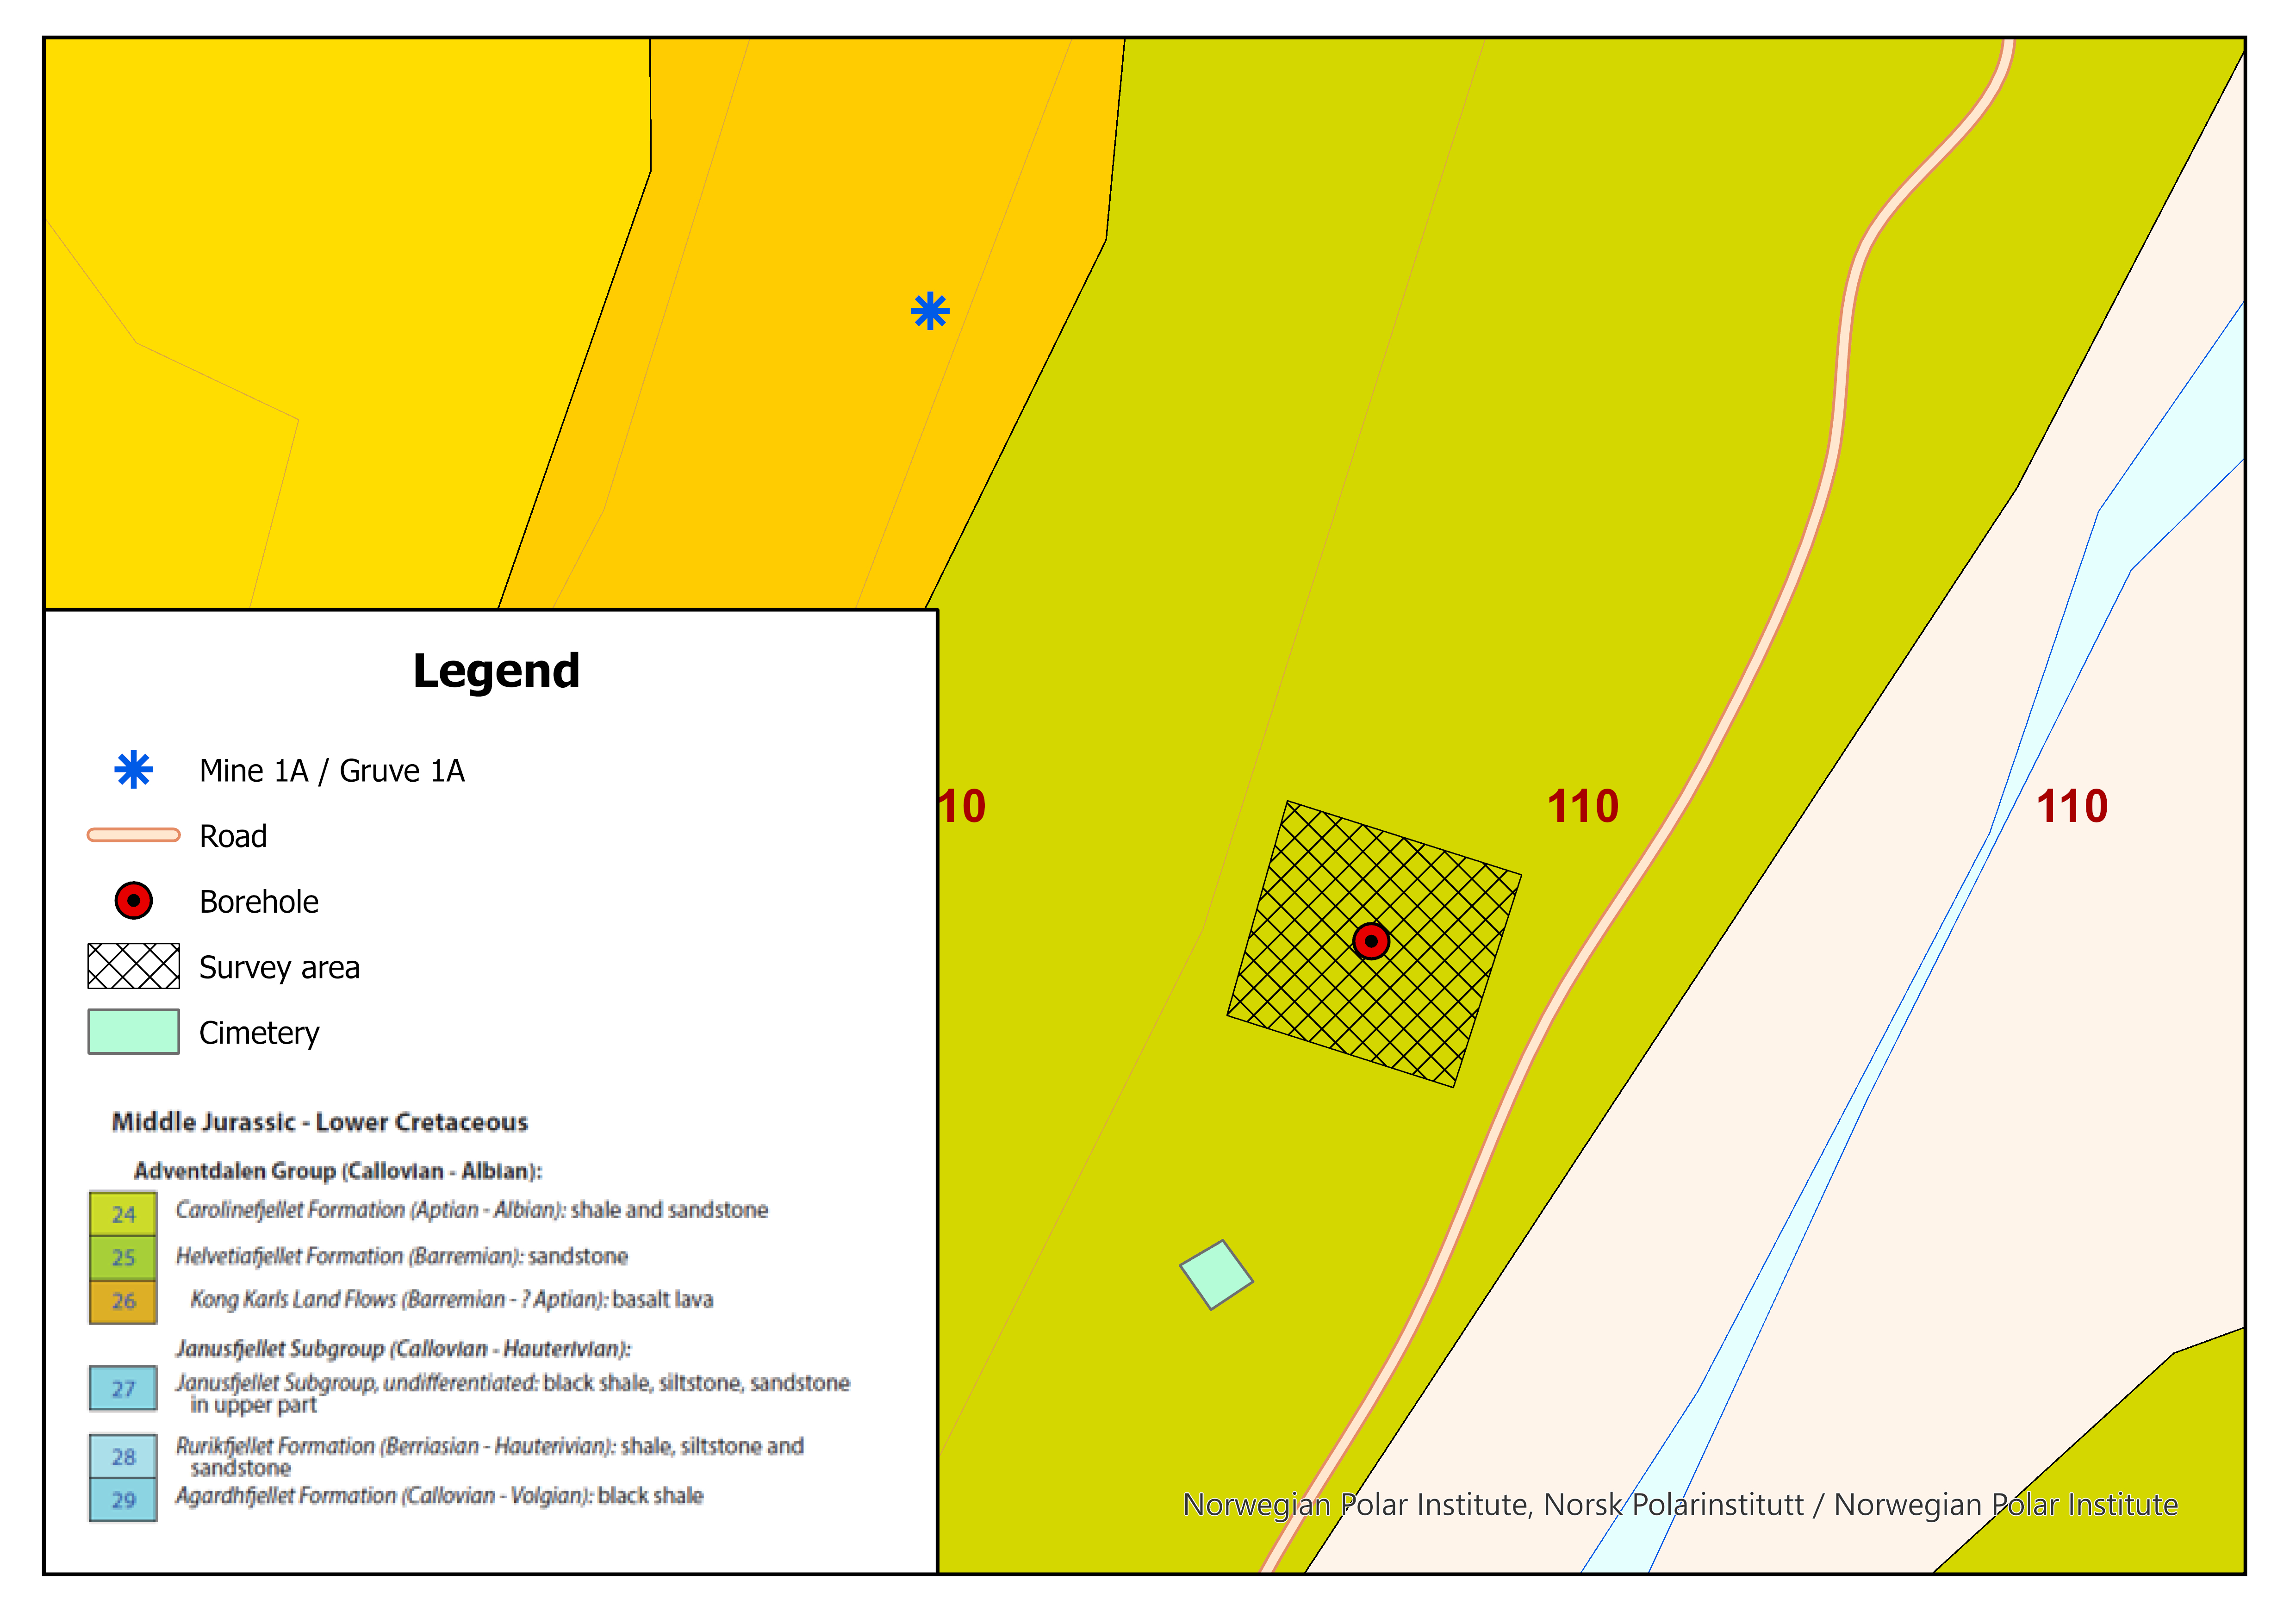
\includegraphics[width=\linewidth]{Images/00_Methodology/GeologicalSituationMap.jpg}
    \caption{Geological background under the survey area \cite{Atakan2015GeoscienceSvalbard}}
    \label{fig:GeologicalBackground}
\end{figure}

\begin{figure}
    \centering
    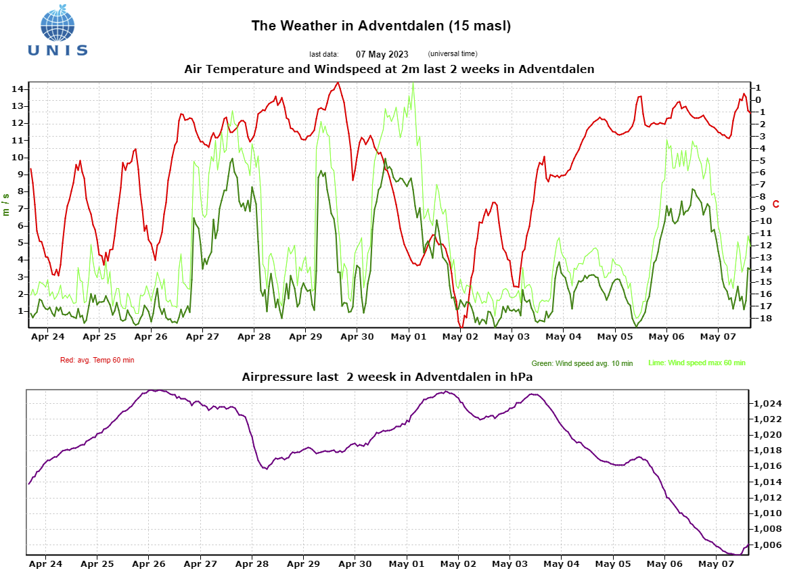
\includegraphics[width=\linewidth]{Images/00_Methodology/WeatherConditions.png}
    \caption{Weather condition around Longyeabyen from the UNIS weather station in Adventdalen between April 24 and May 7 2023}
    \label{fig:weather}
\end{figure}


\paragraph{Weather conditions} The field work takes place in a very perturbed but sunny spring period. The day of the field work, April 28th, the weather was very sunny and warm with a temperature reaching 0.5°C. Figure \ref{fig:weather} shows the history of the weather 2 weeks around the field work. We see an high variability of the temperature (between -18 and 2°C) as well as a high variability of wind.


\paragraph{Safety consideration} In the arctic, safety for field operation is one of the most important concern, even when the field activity are close to the town. According to cold weather, the risk of landslides as it happended in 2018 is very unlikely, because the active layer is still frozen. But a more important concern is avalanches because of the steep slope of the survey and even with a risk of 2 over 5. That's why we have with us all the avalanche safety equipments (avalanche beacon, probe and shovel).
Finally, we stay close to a very crowdy area (cross country ski track), in town and we always stay under phone coverage in case of any emergency.

\paragraph{Planned grid}

The initial plan was to realize a grid as presented in blue on figure \ref{fig:GPRLines} in order to have a resolution under the ground as good as possible. The issue was that to follow the line with the GPS was very hard and the irregularity of the surface increased this complexity. Finally, the main concern was that the initial grid was very ambitious about the physical activity and the long path to be walked.

\begin{figure}[H]
    \centering
    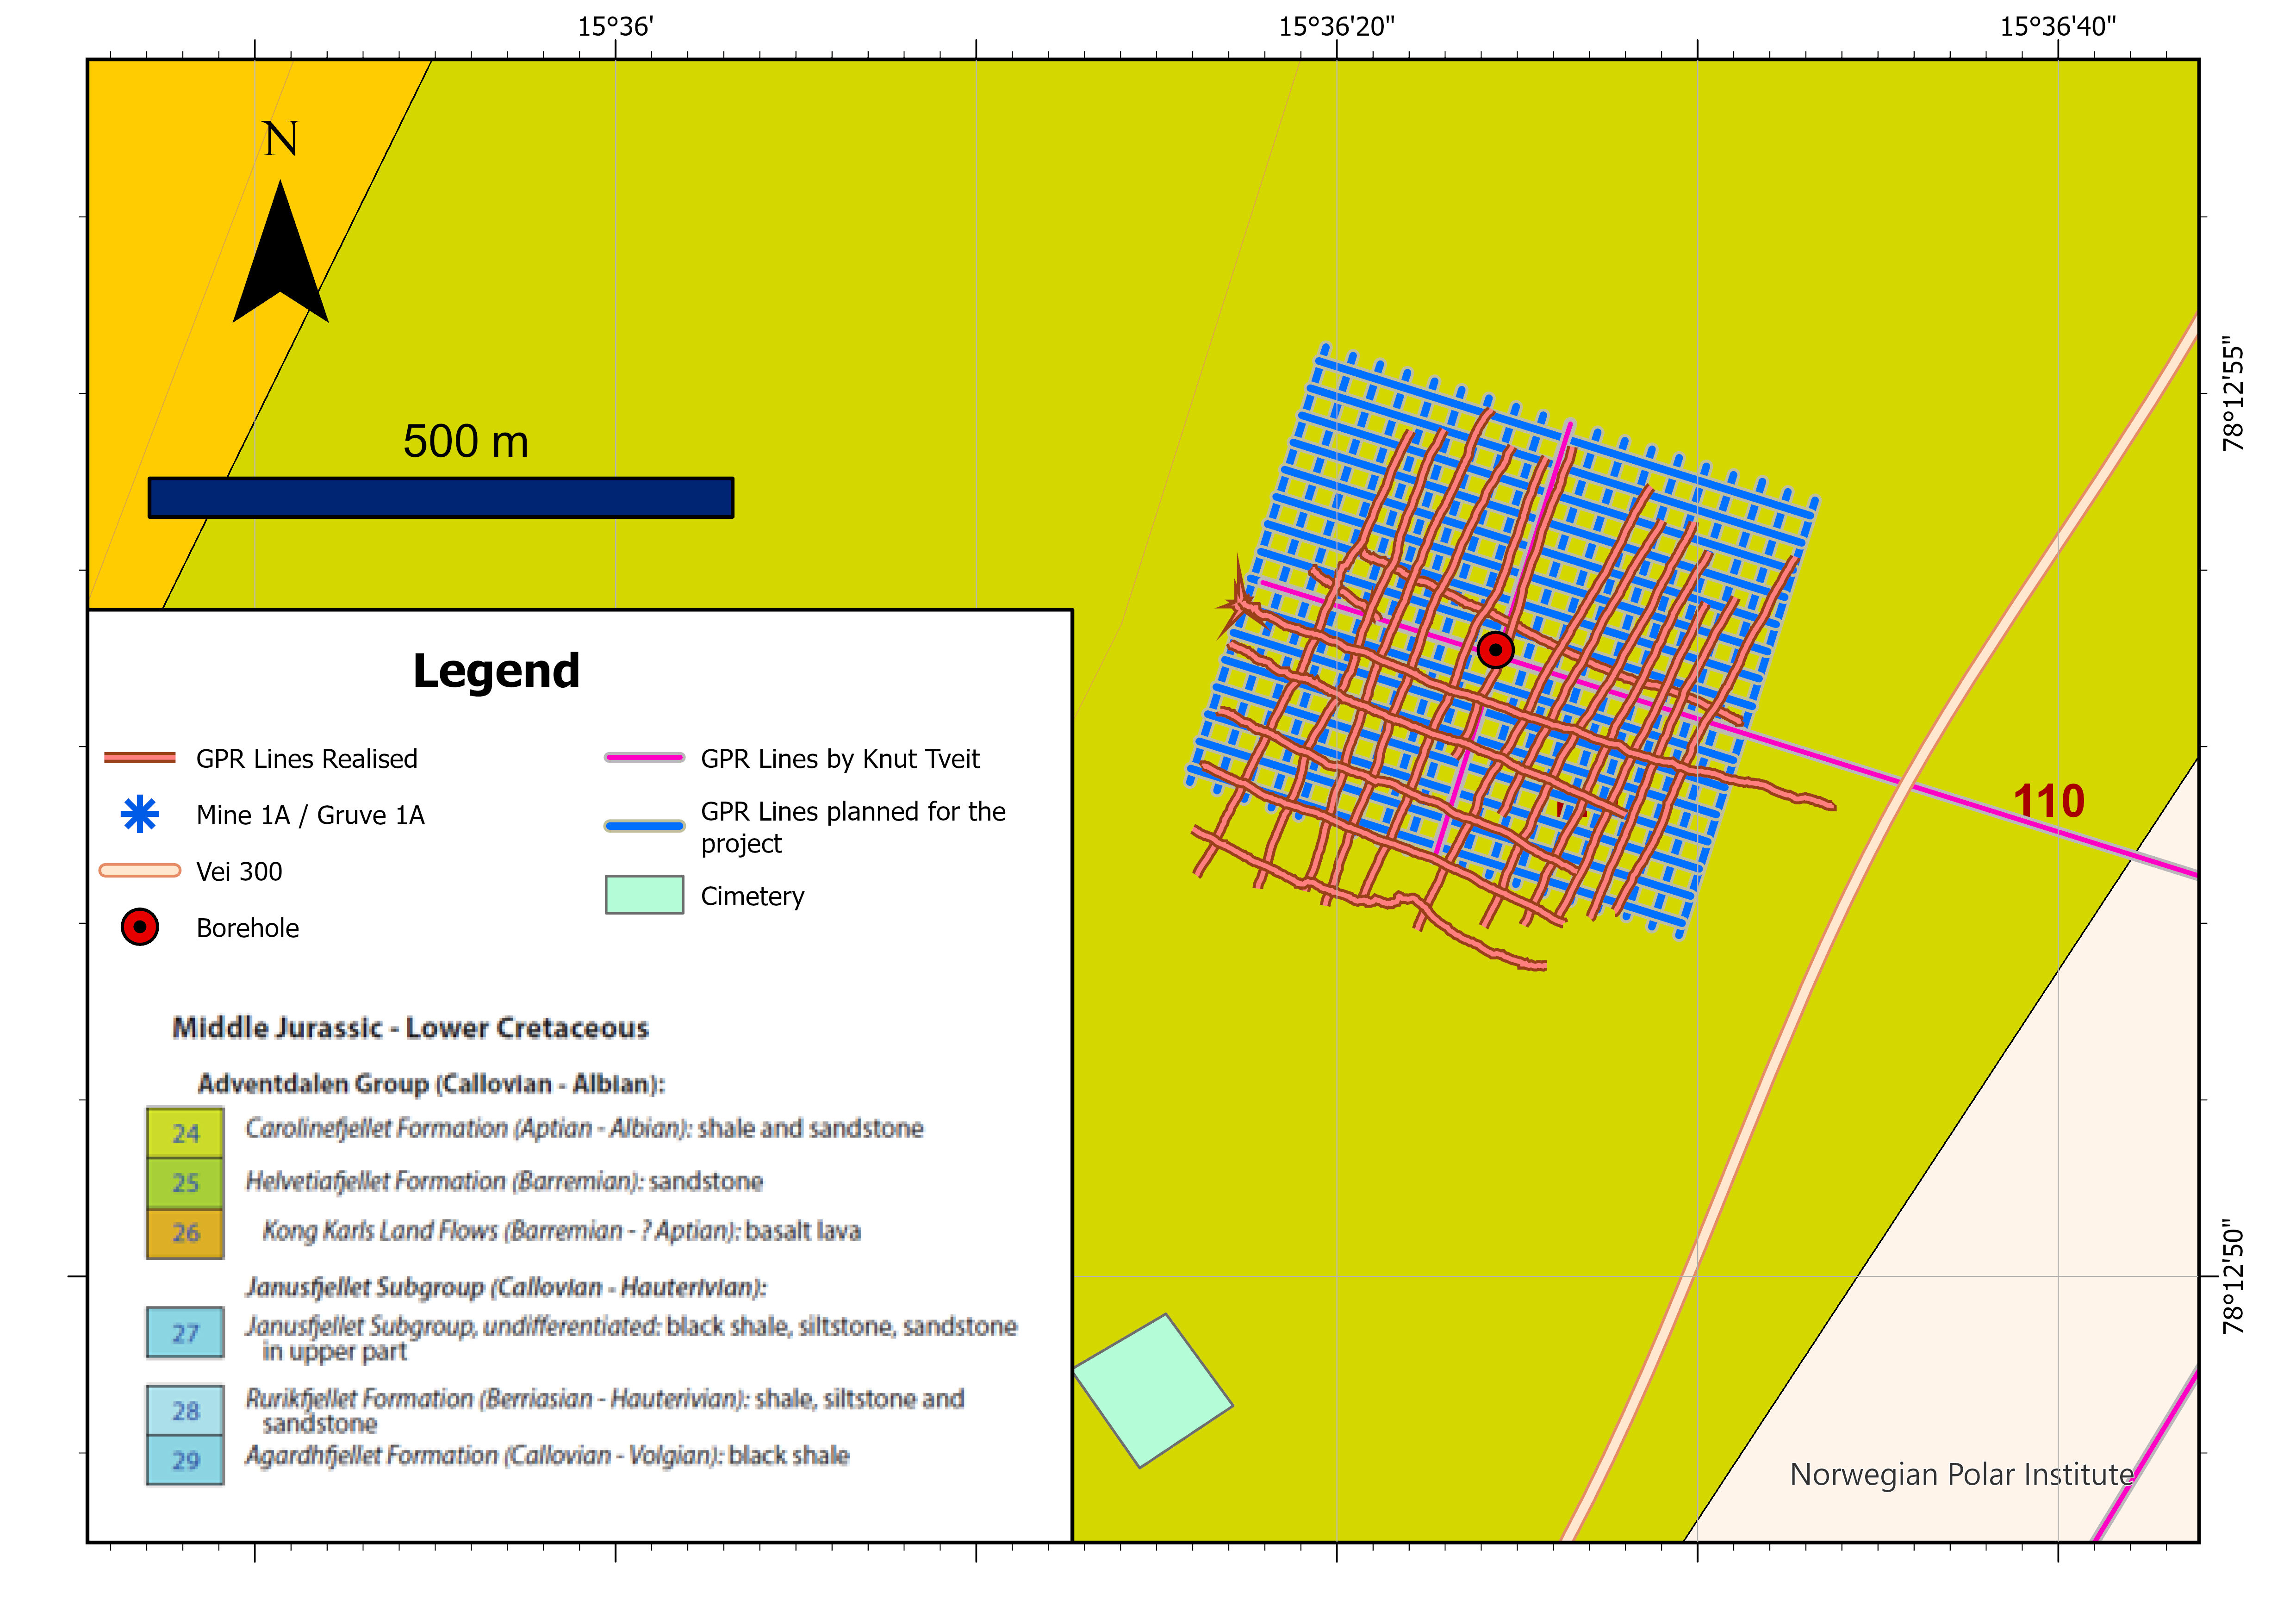
\includegraphics[width=\linewidth]{Images/00_Methodology/GPR LIne.jpg}
    \caption{Lines planned and realised during the main survey}
    \label{fig:GPRLines}
\end{figure}

\subsection{Processing}

The processing in the most important part of the survey, because it will permit to show what is interesting. The easier way is to use the software Ekko Project provided with the GPR by sensor and software.

The first step is to import all the data inside, correct the position of the lines with GPS data and export the data set as CSV as a backup.

After applying a bandpass open from 50 MHz and 150 MHz, we open one of the line and do the following processing :

\begin{enumerate}
    \item Change the color scale in order to keep my eyes alive...
    \item Use the dewow filter in order to remove the electronics wow effect
    \item Apply a gain in order to be able to see some details in the depth. For that part, it's mostly trial and error in order to get a GPR line where we have some contrast everywhere. For our data set, we use the SEC gain which will try to amplify more the deeper layer than the upper layer in order to have an homogeneous picture.
    \item Use a background subtraction to remove the layering created by electronics noise mainly
\end{enumerate}

The next step is to find the velocity using the hyperbolas. Unfortunately, we get only two nice hyperbola due probably to the electric grid which give a velocity around $0.235 m/ns$ where some other very thin and small hyperbola give a velocity closest from $0.109 m/ns$. For all the lines, I choose to use the velocity of $0.235 m/ns$ but I might the wrong one and so the penetration depth should taken only as an indication, because depending of the velocity.

Finally, we apply the same settings to all the lines (knowing that the survey was done in the same place with the same settings) and change the visualisation from depth to elevation to have an idea of the upper geometry of the terrain.
